\documentclass{article}

% list of necessary packages
\usepackage[utf8]{inputenc}
\usepackage{amsfonts, amsmath, amssymb, amsthm}
\usepackage{nicefrac}
%\usepackage{fullpage}
\usepackage[section]{placeins}
\usepackage{url}
\usepackage[english]{babel}
\usepackage{titling}

% list of optional packages
\usepackage{graphicx, subfig}
\usepackage{algpseudocode}
\usepackage{changepage}
\usepackage{xcolor,soul}

% paragraph spacing
\setlength{\parindent}{0pt}
\setlength{\parskip}{8pt}


% table spacing
\def\arraystretch{1.2}


% configuration of header and footer
\pagenumbering{arabic}
\usepackage{fancyhdr} 
\pagestyle{fancy}
\fancyhf{}
\fancyhead[C]{
	{\large {\theauthor} }
}
\fancyfoot[C] {
    { {\thepage} }
}
\renewcommand{\headrulewidth}{0pt} % 0.4pt lined
\setlength{\headheight}{14pt}
\setlength{\headsep}{16pt}
 

\begin{document}
    % config
    \title{Lab: Efficient Algorithms}  % TODO: ganzer Titel war zu lang, so okay?
    \author{Rademacher, Loka}
    \date{\today}

    % super nice header
    \thispagestyle{empty}
    \begin{center}
        \noindent
        \makebox[0pt][l]{Final Report}%
        \makebox[\textwidth][c]{\textbf{University of Bonn}}%
        \makebox[0pt][r]{\thedate}
        
        
        \noindent
        \centerline{\huge \sc \thetitle}
        
        \vspace*{-2pt}
        
        \noindent
        \centerline{\large {\theauthor}}
    \end{center}
    
    
    
    \section{Introduction}
    
    The goal of the lab \textit{Efficient Algorithms and Selected Problems} was to engage with a given problems and state of art algorithms which solve them really well. The problem we are given was path finding on grid graphs and the main algorithm was Jump point search with the pruning technique bounding boxes.
    
    We made an implementation of this algorithms and some similar ones which are frequently used to compare them. The similar algorithms are different variants of jump point search and the well known A star algorithm. On top of implementation the algorithm we have added some tools to visualize the algorithms and to benchmark our algorithm implementation. Our actual implementation is independent from the visualization so that the algorithm is also applicable outside of the visualization environment. The purpose of the visualization environment is to help others understand the algorithm 
    
    The source code of the implementation will be available at \url{https://github.com/dhaunac/lab-jump-point-search} after the final presentation as all our other work relating to the lab.
    
    
    
    \section{Path finding on grid graphs}
    
    Our problem setting is to find the shortest path on a grid graph. So let $G$ be an Euclidean grid graph. It consists of a fixed number of cells which are ordered on an Euclidean grid. Each cell which is not element of $G$ is a so called obstacle. Edges only exist between adjacent cells when both cells are element of $G$. The cost of each edge we travel is determined by the direction of it. An orthogonal edge has cost of $1$ and a diagonal edge has cost of $\sqrt{2}$.
    
    For that cost function on Euclidean grids there are a number of so called heuristic functions. A heuristic function is a function $h : G \times G \rightarrow \mathbb{R}$. The constraint any heuristic function has to fulfill is the admissibility. A admissible heuristic is never overestimating the cost between two points, i.e. for all $a, b \in G$ it holds $c(a, b) \leq h(a,b)$. The other constraint is consistency which says that the heuristic cost between two points is not higher that the heuristic from $a$ to a neighbor of $b$ and the cost from that neighbor to $b$, i.e. $\forall a, b, c: h(a, b) \leq h(a, c) + c(c, b)$. A consistent heuristic is also admissible. If we would use a heuristic which is not admissible then all of our algorithms would not return a correct shortest path. A consistent heuristic improves our running time. All the heuristics we regarded are therefore consistent.
    
    Every problem instance has given two additional points. One of it is the start point and the other the goal point of that instance. This now yields a 4-tuple of grid graph $G$, start point $s$, goal point $g$ and heuristic function $h$. Now the algorithm has to determine the shortest path from start to goal point.\cite{DBLP:conf/aaai/HaraborG11}
    
    
    
    \section{Algorithms}
    \label{sec:algorithms}
    
    The implementation of the following algorithms was the main aspect of the lab task. At first we show an outline of the algorithms so that the reader is familiar with those before discussing implementation issues.
    
    \subsection{A star search $A^\star$ }
    
    In this section we will discuss the $A^\star$ search algorithm. \cite{Astar} The algorithm is basically a natural extension of the Dijkstra algorithm. It consist of an open list of next candidate vertices and a closed list of already processes processes vertices. The open list is usually some kind of priority queue and the closed list is a set.
    
    The algorithm then gets a graph, a cost function and an admissible heuristic function as input. It starts with adding the start node into the open list and then processes a main loop. The main loop extracts the vertex $v$ of the open list with minimum cost and expands all its adjacent vertices. The expansion step check whether the vertices are not in the closed list and if so adds it to the open list with a cost value of the sum from the cost to $v$ and the cost from $v$ to the expanded point. After that add $v$ to the closed list and repeat the main loop. The minimum cost is the sum of the cost value and the heuristic from that point to the goal node. So while progressing closer to the goal point the minimum cost might decrease.
    
    \subsection{Jump point search $JPS$}
    
    Now we will discuss the first paper. \cite{DBLP:conf/aaai/HaraborG11} At first take a look at figure~\ref{fig:symmetricpath} where we can see the behavior of the $A^\star$ algorithm. So for given points there is a high likelihood that there exist a lot of symmetric paths. By symmetric path we refer to path which are equal in terms of the number of edge direction.
    
    \begin{figure}[!htb]
        \centering
        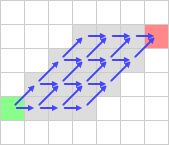
\includegraphics{figures/symmetricpath.png}
        \caption{Different possiblities for the shortest path in $A^\star$ \cite{JPSexplained}}
        \label{fig:symmetricpath}
    \end{figure}
    
    At this point starts the algorithm jump point search. It will avoid all of those symmetric paths by adding a priority to the directions. $JPS$ will always prefer the diagonal step and thus takes it before any orthogonal edge. Additional the algorithm applies a local pruning depending on the direction of the extracted point from the open list. This works in a way that the algorithm will expand in a direction that can be reached with less cost in another way. The obvious direction is the one which is a inversion of the last step. But also going slightly backwards and to a side will result in a not optimal solution. We can observe this for most directions in the two cases diagonal and orthogonal. 
    
    \begin{figure}[!htb]
        \centering
        \subfloat[orthogonal moves. \cite{JPSexplained}]{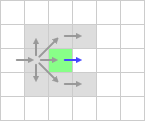
\includegraphics[width=0.4\textwidth]{figures/sm.png}\label{fig:sm}}
        \hfill
        \subfloat[diagonal moves.]{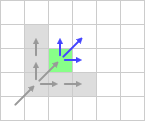
\includegraphics[width=0.4\textwidth]{figures/dm.png}\label{fig:dm}}
        \caption{JPS behavior with no obstacles in sight. \cite{JPSexplained}}
    \end{figure}
    
    So for most points there will be just one expansion point. So instead of pushing each one to the open list we just push those points which have more than one expansion possibilities, because that is an interesting case which have to be decided in a non-trivial way. The skipping of points is called a jump. Jump points are all those points where a jump ends and a new jump can be started. In some cases there are adjacent jump points.
    
    The jump points 
    
    origin from the obstacles in the grid. Every obstacle will remove 
    
    The most important thing to care about is the modifications for obstacles. The improvements mentioned so far will work properly if there are no obstacles on the path. So for any obstacle encountered the algorithms 
    
    \begin{figure}[!htb]
        \centering
        \subfloat[orthogonal moves. \cite{JPSexplained}]{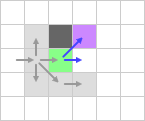
\includegraphics[width=0.4\textwidth]{figures/sm_forced.png}\label{fig:sm_forced}}
        \hfill
        \subfloat[diagonal moves.]{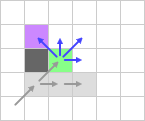
\includegraphics[width=0.4\textwidth]{figures/dm_forced.png}\label{fig:dm_forced}}
        \caption{JPS behavior at encountering obstacles. \cite{JPSexplained}}
    \end{figure}
    
    \begin{figure}[!htb]
        \centering
        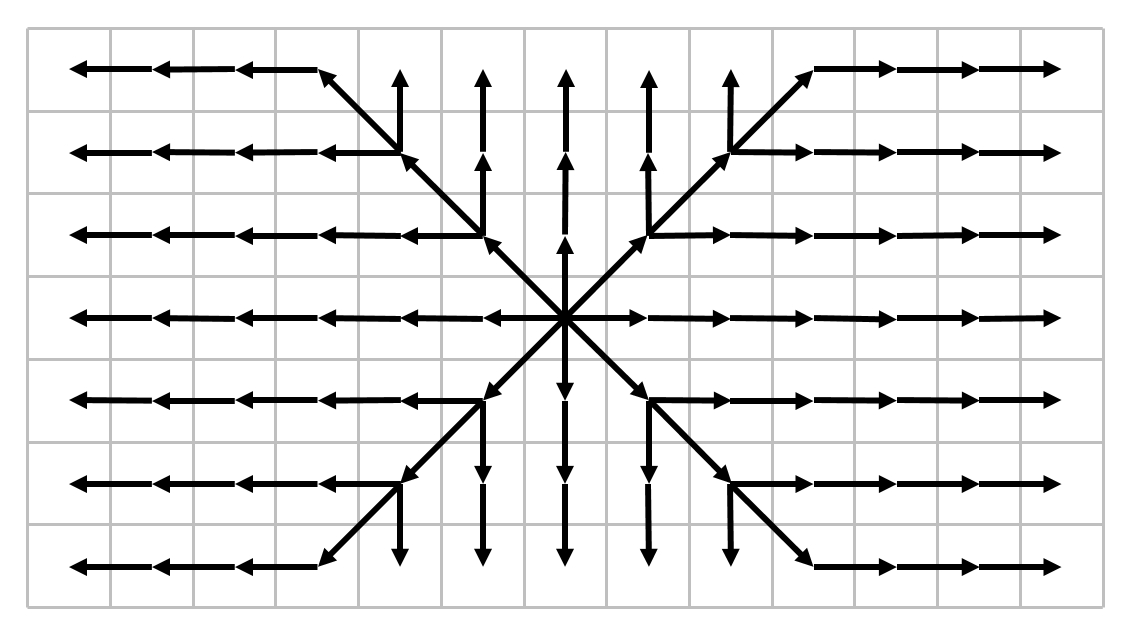
\includegraphics[width=\textwidth]{figures/jps_strategy.png}
        \caption{Natural order of exploration in $JPS$}
        \label{fig:pathorder}
    \end{figure}
    
    
    
    \subsection{Jump point search Improvements $JPS^+$}
    
    There is an improvement of $JPS$ called $JPS^+$. \cite{DBLP:conf/aips/HaraborG14}
    
    
    
    \subsection{Bounding boxes pruning $BB$}
    
    Bounding boxes is a pruning technique that can be applied to lot of different path finding algorithms. \cite{DBLP:conf/aaai/RabinS16} The pruning requires some preprosessing which can be done offline, i.e. before the actual start and goal point are known.
    
    For each pair of points and direction we have a dedicated bounding box. This box consists of all points which are can be reached optimally on a path from that given point. The box itself is the smallest geometric container, in this case a square, to have every of those points inside. This implies that any point outside the box will be pruned since they will not help finding an optimal path.
    
    The bounding depends on the underlying algorithms, in case of $A^\star$ and $JPS$ it is sufficient to have minimum and maximum values for the X and Y coordinates. For $A^\star$ we can determine a predecessor $p$ for the point $v$ by inverting the direction. Then the bounding box of the point consists of all points which have a shortest path from $p$ to those points using $v$ as intermediate point. For $JPS$ we can go even further and use the knowledge of our jump points and natural ordering. Here the pruning will be even more effective which can be observed in our visualization of the algorithm.
    
    \begin{figure}[!htb]
        \centering
        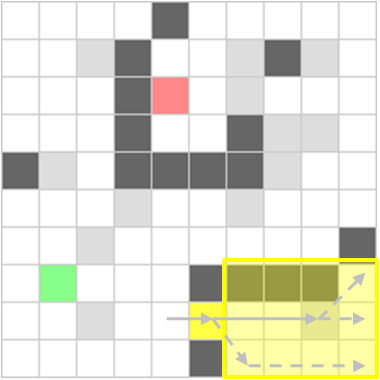
\includegraphics{figures/bounding_boxes.png}
        \caption{Natural order of exploration in $JPS$}
        \label{fig:bounding_boxes}
    \end{figure}
    
    
    
    \subsection{Comparison}
    
    TODO: Optionales Vergleichen von Bilder der Ergebnissen, weiß aber noch nicht, ob das viel Sinn ergibt
    
    
    
    \section{Visualization and user interface}
    
    The visualization is the was the second substantial aspect of our work. To begin we will explain the basic working of the user interface. At first one can use the \textit{File} menu to load any map. There are a number of different possibilities to create a random map satisfying a specific layout, for example perfect mazes or random rooms connected in a selected way. The next menu is \textit{Edit} where one choose to edit the map or the algorithm settings. We offer $A^\star$, $JPS$, $JPS^+$ and $JPS+BB$ which are explained in section~\ref{sec:algorithms}. On top of that one can modify each of those algorithms by choosing a heuristic and a moving rule. The heuristic modification leads into situations where different candidates of the open list will be explored. The change in the moving rule offers interesting observations when used with some kinds of jump point search and shows also the limits of jump point search. Then the user is supposed to pick locations for the start and goal point. Then the algorithm can be run after some prepossessing if necessary. We have separate steps for those actions, so one can easily modify the algorithm settings and see the changes after running the other algorithm settings.
    
    The visualization will show the result of the algorithms. The red line between the chosen start and goal point indicates the shortest path. We have different colors for points which are in the open list or closed list. Every type of points can be shown or hidden by using the \textit{View} menu.
    
    The Java implementation is written using JavaFX, the successor of Swing.
    
    TODO: Eventuell noch ein Screenshot von der super geilen UI einfügen
    
    
    
    \section{Approach}
    TODO: Eine Beschreibung unserer Vorgehensweise ist bestimmmt noch ganz interessant
    
    
    
    \section{Implementation issues}
    TODO: Hier sollen ein paar konkrete Beispiele hin, wo wir längere Zeit dran gearbeitet haben
    
    TODO: ein Bild von der Direction Uhr erstellen
    
    
    
    \section{Conclusion}
    TODO: Hier könnten ein paar Plots stehen aus den benchmark Ergebnissen, die wir haben (?)
    
    
    
    \bibliographystyle{alpha}
    \bibliography{references}
\end{document}
